\section{State of the art image reconstruction}
Long time research.
Field that is cracking up

Major cycle architecture.
Discuss the algorithms 
Split into two parts. We discuss the gridding first. It is responsible

\subsection{Gridding algorithms}
Biggest part is $w$-term, how to handle it efficiently. Important for wide field of view observation.
Meaning really important for the SKA precursors like MeerKAT and MWA, and for the eventual SKA instruments.

(show the problem of $w$-component)

Accuracy and speed.

Faceting.

$w$-projection algorithm \cite{cornwell2008noncoplanar}
Convolution in the Fourier domain.




 The WSCLEAN \cite{offringa2014wsclean} did a large part.

More recently, the Image domain gridding algorithm has been developed \cite{veenboer2017image}. Which can put it on the gpu, along with handling more DDE's.

\subsubsection{$w$-stacking}
Idea of $w$-stacking, creating stacks of $w$-stack. So each visibility with similar $w$-component is in the same stack. Turns out we can then move

\subsubsection{Image Domain Gridder}
Recently developed\cite{veenboer2017image}. It works by partitioning the input visibilities into subgrids, and then calculates the interpolation and $w$-correction for each subgrid.

Called image domain, because a convolution in Fourier space is a multiplication in image space, interpolation kernels can are applied in image space. uses the idea of subgrids.

\begin{figure}[h]
	\centering
	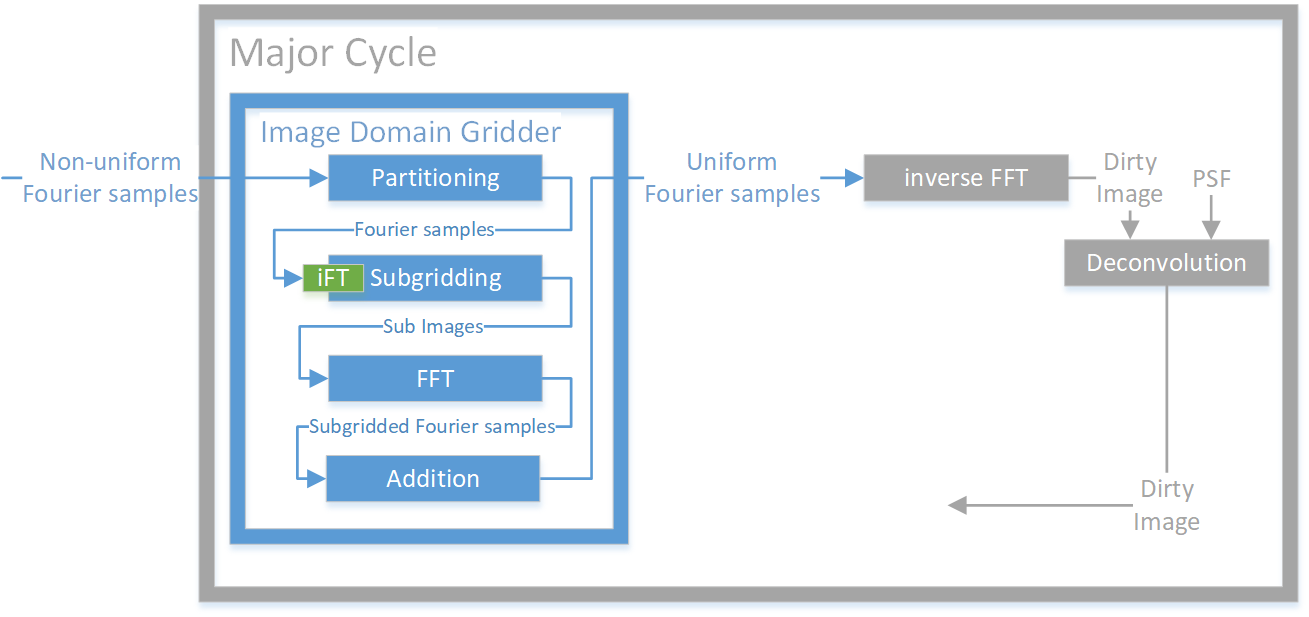
\includegraphics[width=0.80\linewidth]{./chapters/03.distribution/idg/major-minor-idg.png}
	\caption{Image Domain Gridder in the Major Cycle Architecture}
	\label{distribution:idg:system}
\end{figure}

Algorithm
\begin{figure}[h]
	\centering
	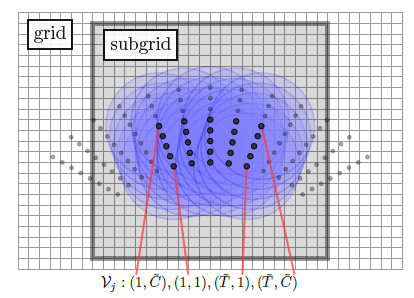
\includegraphics[width=0.40\linewidth]{./chapters/03.distribution/idg/subgrid.png}
	\caption{Subgrid}
	\label{distribution:idg:subgrid}
\end{figure}

\begin{figure}[h]
	\centering
	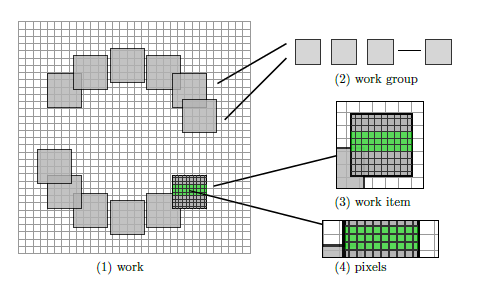
\includegraphics[width=0.40\linewidth]{./chapters/03.distribution/idg/paralellization.png}
	\caption{parallel}
	\label{distribution:idg:parallel}
\end{figure}

\begin{figure}[h]
	\centering
	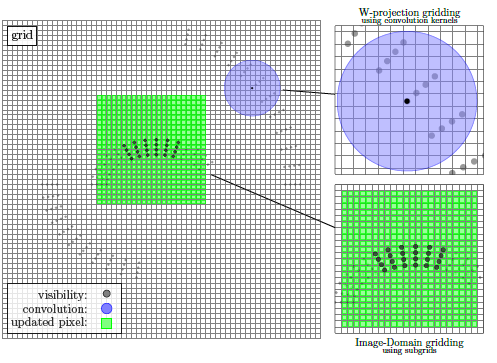
\includegraphics[width=0.40\linewidth]{./chapters/03.distribution/idg/idg0.png}
	\caption{Image Domain Gridder in the Major Cycle Architecture}
	\label{distribution:idg:idg0}
\end{figure}


\subsection{Deconvolution algorithms}
\subsubsection{MS-MFS-CLEAN}
CLEAN basic \cite{hogbom1974aperture}.

Latest variants for multiscale and multi frequency CLEAN (MS-MFS-CLEAN)\cite{rau2011multi}.

Current state-of-the-art

\subsection{Reconstruction algorithms which are not based on the deconvolution}
SARA










